\documentclass{VUMIFPSbakalaurinis}
\usepackage{algorithmicx}
\usepackage{algorithm}
\usepackage{algpseudocode}
\usepackage{amsfonts}
\usepackage{amsmath}
\usepackage{bm}
\usepackage{caption}
\usepackage{color}
\usepackage{float}
\usepackage{graphicx}
\usepackage{listings}
\usepackage{subfig}
\usepackage{wrapfig}
\usepackage[table,xcdraw]{xcolor}
\usepackage{enumitem}
\usepackage{longtable}
\setitemize{noitemsep,topsep=0pt,parsep=0pt,partopsep=0pt}
\setenumerate{noitemsep,topsep=0pt,parsep=0pt,partopsep=0pt}

\hbadness=100000
% Titulinio aprašas
\university{Vilniaus universitetas}
\faculty{Matematikos ir informatikos fakultetas}
\department{Programų sistemų studijų programa}
\papertype{Mokslo tiriamasis darbas III}
\title{Srautinio apdorojimo sistemų balansavimas taikant mašininį mokymąsi}
\titleineng{Balancing stream processing systems using machine learning}
\author{Vytautas Žilinas}
\supervisor{Andrius Adamonis}
\reviewer{Prof. dr. Aistis Raudys}
\date{Vilnius – \the\year}

% Nustatymai
% \setmainfont{Palemonas}   % Pakeisti teksto šriftą į Palemonas (turi būti įdiegtas sistemoje)
\bibliography{bibliografija}

\begin{document} 
\maketitle

\cleardoublepage\pagenumbering{arabic}
\setcounter{page}{2}

\tableofcontents

\sectionnonum{Įvadas}

Realaus laiko duomenų apdorojimas (angl. real–time data processing) yra jau senai nagrinėjamas kaip vienas iš būdų apdoroti didelių kiekių duomenis (angl. Big data). Viena iš didelių duomenų apdororojimo tipinių architektūrų yra srautinis apdorojimas. Srautinis duomenų apdorojimas (angl. stream processing) – lygiagrečių programų kūrimo modelis, pasireiškiantis sintaksiškai sujungiant nuoseklius skaičiavimo komponentus srautais, kad kiekvienas komponentas galėtų skaičiuoti savarankiškai \cite{shortstreamproc}. 

Yra keli pagrindiniai srautinio apdorojimo varikliai: „Apache Storm“, „Apache Spark“, „Heron“ ir kiti. „Apache Storm“ ir „Heron“ apdoroja duomenis duomenų srautais, o „Apache Spark“ mikro–paketais \cite{karau2015learning}. „Heron“ srautinio apdorojimo variklis, buvo išleistas „Twitter“ įmonės 2016 metais kaip patobulinta alternatyva „Apache Storm“ srautinio apdorojimo varikliui \cite{openSourcing}. Šiame darbe bus naudojamas „Heron“, kadangi tai yra naujesnis ir greitesnis srautinio apdorojimo variklis nei „Apache Storm“ \cite{twitterHeron}. 

Srautinio apdorojimo sistemų balansavimas (angl. auto–tuning) – tai sistemos konfigūracijos valdymas siekiant užtikrinti geriausią resursų išnaudojimą – duomenų apdorojimas neprarandant greičio, bet ir naudojant tik reikiamą kiekį resursų. Kadangi srautinio apdorojimo sistemų komponentai yra kuriami kaip lygiagretus skaičiavimo elementai, todėl jie gali būti plečiami horizontaliai ir vertikaliai \cite{shortstreamproc} keičiant sistemų konfigūraciją. Tačiau lygiagrečių elementų kiekio keitimas nėra vienintelis būdas optimizuoti resursų išnaudojimą. Kiekvienas variklis turi savo rinkinį konfigūruojamų elementų. Pavyzdžiui, darbe naudojamas „Heron“ variklis leidžia optimizuoti sistemas naudojant 56 konfigūruojamus parametrus \cite{configDocument}.

Yra skirtingi būdai kaip gali būti parenkama tinkama konfigūracija. Kadangi srautinio apdorojimo sistemų apkrovos gali būti skirtingų pobūdžių (duomenų kiekis, skaičiavimų sudėtingumas, nereguliari apkrova), o inžinieriai kurdami ir konfigūruodami taikomasias sistemas išbando tik kelis derinius ir pasirenka labiausiai tinkanti \cite{selfRegulatingStreaming}, lieka daug skirtingų neišbandytų konfigūracijos variacijų. Optimalios konfigūracijos suradimas yra NP sudėtingumo problema \cite{automateTuning}, kadangi žmonėms yra sunku suvokti didelį kiekį konfigūracijos variacijų. 
Vienas iš būdų automatiškai valdyti konfigūraciją buvo pasiūlytas 2017 metų straipsnyje „Dhalion: self–regulating stream processing in heron“, kuriame autoriai aprašo savo sukurtą sprendimą „Dhalion“, kuris konfigūruoja „Heron“ srautinio apdorojimo sistemas pagal esamą apkrova ir turimus resursus, tai yra jei apdorojimo elementų išnaudojimas išauga virš 100\%, „Dhalion“ padidina lygiagrečiai dirbančių apdorojimo elementų kiekį \cite{dhalion}. Tačiau toks sprendimas leidžia reguliuoti tik elementų lygiagretumą ir tai daro tik reaktyviai.

Vienas iš naujausių būdų balansuoti srautinio apdorojimo sistemas – mašininis mokymasis. Vienas iš tokių bandymų aprašytas 2018 metų straipsnyje „Auto–tuning Distributed Stream Processing Systems using Reinforcement Learning“\cite{vaquero2018autotuning} kuriame atliktas tyrimas – „Apache Spark“ sistemos balansavimui naudojamas skatinamojo mokymo REINFORCE algoritmas, kuris, pagal dabartinę konfigūraciją ir renkamas metrikas, keitė srautinio apdorojimo sistemos konfigūracijos parametrus. Šiame tyrime pasiūlytas sprendimas, naudojantis mašininį mokymąsi, suranda efektyvesne konfigūraciją per trumpesnį laiką nei žmonės, o tokiu būdu išskaičiuotą konfigūraciją naudojanti sistema pasiekia 60–70\% mažesnį vėlinimą, nei naudojanti ekspertų rankiniu būdu nustatytą konfigūraciją. \cite{vaquero2018autotuning}. Šiame darbe naudojamas „Heron“ variklis leidžia prie savęs prijungti sukurtą išorinę metrikų surinkimo programą, kuri gali rinkti tokias sistemų metrikas kaip: naudojama RAM atmintis, CPU apkrova, komponentų paralelizmas ir kitas, kurios gali būti naudojamos balansavimui. 

Skatinamasis mokymasis yra vienas iš mašininio mokymosi tipų. Šis mokymasis skiriasi nuo kitų, nes nereikia turėti duomenų apmokymui, o programos mokosi darydamos bandymus ir klysdamos. Vienas iš pagrindinių privalumų naudojant skatinamąjį mokymąsi balansavimui – nereikia turėti išankstinių duomenų apmokymui, kas leidžia jį paprasčiau pritaikyti skirtingoms srautinio apdorojimo sistemų apkrovoms. Tačiau tokio tipo mašininis mokymasis turi ir problemų: sudėtinga aprašyti tinkamos konfigūracijos apdovanojimo (angl. reward) funkciją ir balansą tarp tyrinėjimo ir išnaudojimo tam, kad nebūtų patiriami nuostoliai \cite{selfRegulatingStreaming}.

Yra sukurta daug skatinamojo mokymosi algoritmų (Monte Carlo, Q–learning, Deep Q Network ir kiti), šiame darbe jie apžvelgti, pasirinkti ir pritaikytas išsikeltam uždaviniui. 

Magistro darbo tikslas: Ištirti mašininio mokymosi tinkamumą srautinio apdorojimo sistemų balansavimui. 

Magistro darbo uždaviniai:
\begin{enumerate}
    \item Sudaryti srautinio apdorojimo sistemų balansavimo modelį ir nustatyti valdymo metrikas ir jų siekiamas reikšmes, kurios bus naudojamos eksperimentinėje sistemoje.
    \item Parinkti skatinamojo mokymosi algoritmą eksperimentui, atsirenkant iš algoritmų, aprašomų literatūroje.
    \item Sukurti eksperimentinį sprendimą su pasirinktu algoritmu ir atlikti eksperimentus.
    \item Palyginti eksperimento rezultatus su alternatyvomis – „Heron“ su standartine konfigūracija bei „Heron“ balansavimas pritaikius REINFORCE algoritmą. 
\end{enumerate}
Antroje magistro darbo dalyje atlikta literatūros analizė, sudarytas balansavimo modelis ir parinkti skatinamojo mokymosi algoritmai, o šiame mokslo tyriamajame darbe – trečio magistro darbo dalyje – siekta tikslo : apibrėžti darbo metodą ir sukurti bei pagrįsti algoritmą, kuris bus naudojamas eksperimentui. Ir įgyvendinti šie uždaviniai:
\begin{enumerate}
    \item Apibrėžti algoritmą srautinio apdorojimo sistemų balansavimui naudojanti Deep Q Network ir Soft Actor Critic skatinamojo mokymosi algoritmus.
    \item Apibrėžti eksperimento eigą ir altenatyvius sprendimus, kurių rezultatai bus naudojami algortimo įvertinimui. 
\end{enumerate}

\section{Srautinės duomenų apdrojimo sistemos, valdomos mašininiu mokymusi, modelis}

Tyrime nagrinėjamas srautinės sistemos, balanasuojamos mašininių mokymų, modelis (\ref{dataflow} pav.) susidaro iš trijų pagrindinių elementų: srautinio duomenų apdorojimo sistemos, srautinio duomenų apdorojimo platformos ir valdymo sistemos. 
\subsection{Modelis}
\begin{figure}[H]
    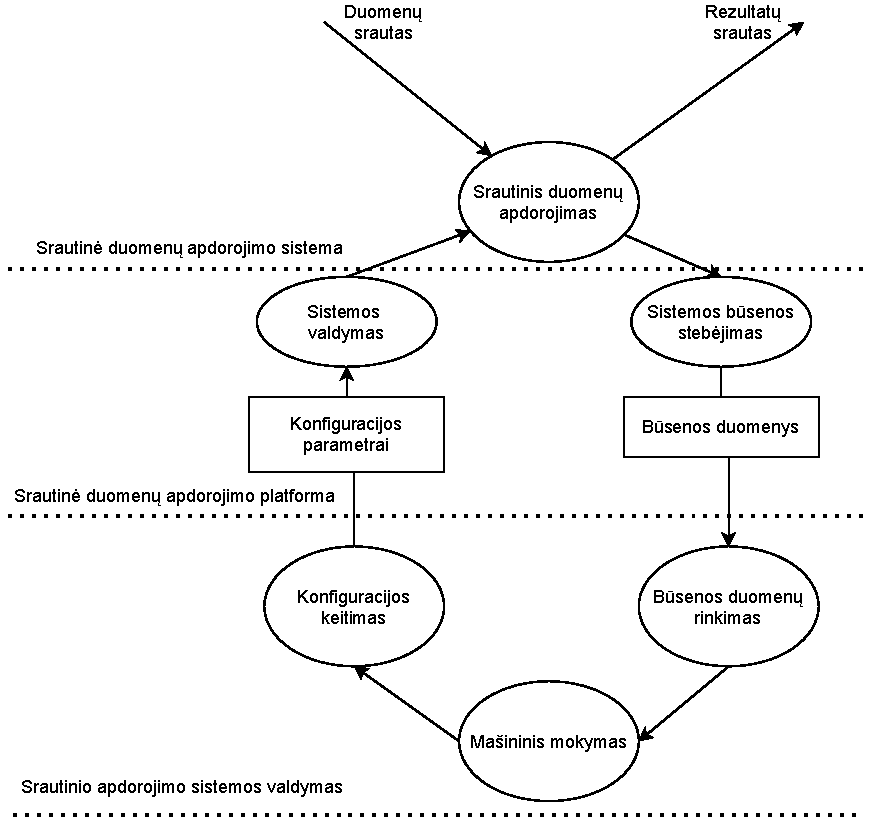
\includegraphics[width=15cm]{img/DataFlow.pdf}
    \caption{Srautinės aprodojimo sistemos modelis}
    \label{dataflow}
\end{figure} 
Srautinės duomenų apdorojimo sistemos modėlį sudaro šie elementai:
\begin{itemize}
    \item Duomenų srautas - duomenys patenkantys į srautinio apdorojimo sistemą nepertraukiamu srautu, iš anksto nežinomu greičiu ir nekontroliuojamu kiekiu.
    \item Srautinis duomenų apdorojimos - srautinio duomenų apdorojimo sistemą, atliekanti skaičiavimus su duomenim ateinančiu iš Duomenų srauto. Tyrime naudojama Heron srautinio apdorojimo sistemos pasižymį individualiais skaičiavimo komponentais, kurie skaičiuoja kiekvieną patenkantį duomenį ir yra pararšyti užtikrinant lygiagretumą kiekvienam komponentui.
    \item Rezultatų srautas - duomenys apdoroti srautinio duomenų apdorojimo ir perduoti iš paskutinio skaičiavimo komponento į kitas sistemas.
\end{itemize}
Srautinio apdorojimo sistemų platforma turi šiuos elementus:
\begin{itemize}
    \item Srautini duomenų apdorojimą.
    \item Sistemos būsenos stebėjimą - srautinio apdorojimo platformos sistema renkanti srautinio apdorojimo sistemų veikimo metrikas ir šias metrikas atskleidžianti į išorę. Tyrime naudojama Heron platforma metrikas pateikia kiekvienam skaičiavimo komponetui individualiai per HTTP protokolą arba į naudotojo pateiktą metrikų surinkimo sistemą.
    \item Būsenos duomenys - tai metrikos vaizduojančios kiekvienos srautinio apdorojimo sistemos skaičiavimo komponentų pagrindinius veikimo rodiklius, tokius kaip vėlinimas, pralaidumas, apkrovos ir t.t.
    \item Konfiguracijos parametrai - tai konfiguracijos rinkinys kurį apibrežia srautinio apdorojimo platforma. Šie konfiguracijos paramentrai apibrežia ir bendrą sistemos veikimą ir yra parametrų skirtų individualiems skaičiavimo komponentams. Tyrime naudojama Heron platforma apibrežia ir valdo visus konfiguracijos parametrus.
    \item Sistemos valdymas - konfiguracijos parametrų pateikimas į srautinio apdorojimo plattformą. Šie konfiguracijos parametrai nurodo srautinės apdorojimo sistemos ir jos skaičiavimo komponentų veikimą. Tyrime naudojama Heron platformą leidžia pateikti konfiguracijos parametrus per komandine eilutę. Pateikus konfiguracija platforma sustabdo srautinę apdorojimo sistemą, atnaujina jos konfiguraciją ir paleidžia sistemą iš naujo. Kai sistema sustabdoma, tai pat nustojama ir skaityti duomenis iš duomenų srauto, o paleidus duomenis pradedami skaityti toliau.
\end{itemize}
Srautinio apdorojimo sistemos valdymo elementai susidaro iš:
\begin{itemize}
    \item Būsenos duomenų rinkimo - tai sistema renkanti duomenis apie srautinės apdorojimo sistemos būseną iš srautinės apdorojimo platformos. Ši sistema atsakinga už aktualių metriku surinkimą, kurios naudojamos suformuoti vaizdą apie srautinės sistemos būseną.
    \item Mašininio mokymosi - sistema, kurį gauna srautinės apdorojimo sistemos būsenos duomenis ir pagal tai apskaičiuoja naujas konfiguracijos parametrų reikšmes. Tyrime naudojamas skatinamasis mašininis mokymasis, kuris pastoviai bando pagerinti sistemos būseną atnaujinant konfiguracijos ir mokosi iš padarytų sprendimų.
    \item Konfiguracijos keitimo - sistema priimanti atnaujintus konfiguracijos parametrus ir pateikianti juos į srautinio apdorojimo platformą. 
\end{itemize}

Visumoje \ref{dataflow} paveikslėlis apibrežia duomenų judėjimą reikalinga srautinio duomenų apdorojimo sistemos valdymui. Srautinio apdorojimo sistema yra pagrindinis elementas atsakingas už patį duomenų apdorojimą ir veikia nepriklausomai nuo kitų elementų modelyje. Srautinio apdorojimo platforma talpina ir palaiko srautinio apdorojimo sistemas, taip pat suteikia prieiga gauti informaciją apie srautinio apdorojimo sistemų būsena bei suteikia galimybę valdyti srautinio apdorojimo sistemas. Srautinio apdorojimo sistemų valdymo elementai atsakingi už srautinės apdorojimo sistemos konfiguracijos keitimą pagal surinktus būsenos duomenis.

\subsection{Keičiami konfiguracijos parametrai}

Norint koreguoti konfiguracijos parametrus reikia siųsti atnaujinimo komandą į Heron komandinės eilutė įrankį (toliau Heron CLI). Peteikus konfiguracijos parametrus Heron platformą perkrauna srautinio apdorojimo sistema su naujais parametrais. 
Vienas iš pagrindinių srautinės apdorojimo sistemos konfiguracijos parametrų yra skaičiavimo komponentų lygiagretumas nurodantis kiek paleidžiama tam tikro komponento instancijų. Taip pat tai yra vienintelis keičiamas konfiguracijos elementas, kuris priklauso nuo srautinio apdorojimo sistemos.

Visi kiti konfiguravimo parametrai\cite{configDocument},  kurie taip pat yra keičiami balansavimo metu pateikti \ref{param–table} lentelėje:

\begin{longtable}{|p{0.59\linewidth}|p{0.41\linewidth}|}
    \caption{Keičiami konfiguracijos parametrai}
    \label{param–table}\\
    \hline
    \rowcolor[HTML]{C0C0C0} 
    Parametras                                              & Paaiškinimas                                                                                 \\ \hline
    \endfirsthead
    %
    \endhead
    %
    component–parallelism=[skaičiavimo komponento pavadinimas]            & Tam tikro skaičiavimo komponento lygiagretumas                                 \\ \hline
    heron.instance.tuning.expected.bolt.read.queue.size                   & Numatomas skaitomos eilės dydis Bolt tipo komponentuose                        \\ \hline
    heron.instance.tuning.expected.bolt.write.queue.size                  & Numatomas rašomos eilės dydis Bolt tipo komponentuose                          \\ \hline
    heron.instance.tuning.expected.spout.read.queue.size                  & Numatomas skaitomos eilės dydis Spout tipo komponentuose                       \\ \hline
    heron.instance.tuning.expected.spout.write.queue.size                 & Numatomas rašomos eilės dydis Spout tipo komponentuose                         \\ \hline
    heron.instance.set.data.tuple.capacity                                & Didžiausias kiekis kortežų sugrupuottu vienoje žinutėje                        \\ \hline
    heron.instance.emit.batch.time.ms                                     & Didžiausias laikas Spout tipo komponentui išsiųsti gautą kortežą               \\ \hline
    heron.instance.emit.batch.size.bytes                                  & Didžiausias partijos dydis Spout tipo komponentui išsiųsti gautą kortežą       \\ \hline
    heron.instance.execute.batch.time.ms                                  & Didžiausias laikas Bolt tipo komponentui apdoroti gautą kortežą                \\ \hline
    heron.instance.execute.batch.size.bytes                               & Didžiausias partijos dydis Bolt tipo komponentui apdoroti gautą kortežą        \\ \hline
    heron.instance.internal.bolt.read.queue.capacity                      & Skaitomos eilės dydis Bolt komponentams                                        \\ \hline
    heron.instance.internal.bolt.write.queue.capacity                     & Rašomos eilės dydis Bolt komponentams                                          \\ \hline
    heron.instance.internal.spout.read.queue.capacity                     & Skaitomos eilės dydis Spout komponentams                                       \\ \hline
    heron.instance.internal.spout.write.queue.capacity                    & Rašomos eilės dydis Spout komponentams                                         \\ \hline
    heron.api.config.topology\_container\_max\_ram\_hint                  & Daugiausiai operatyvios atminties kiekio konteineriui išskyrimo užuomina       \\ \hline
    heron.api.config.topology\_container\_max\_cpu\_hint                  & Daugiausiai procesoriaus pajegumo konteineriui išskyrimo užuomina              \\ \hline
    heron.api.config.topology\_container\_max\_disk\_hint                 & Daugiausiai kietojo disko atminties kiekio konteineriui  išskyrimo užuomina    \\ \hline
    heron.api.config.topology\_container\_padding\_percentage             & Užuominų galimą paklaidą                                                       \\ \hline
\end{longtable}

\subsection{Naudojamos metrikos}
Metrikos iš Heron srautinio apdorojimo sistemų gali būti pasiektos keliais skirtingais būdais: darant užklausą į Heron API, skaitant iš tekstinio failo, kurį pildo Heron platformą, sukurti savo metrikų skaitymo priedą ir pateikti jį į Heron platformą prieš ją paleidžiant. Visos metrikos yra saugomos srautinio apdorojimo sistemos kiekvienam skaičiavimo komponentui. 

\ref{metrics–table} lentelėje aprašytos metrikos yra standartinės visiems Heron srautinio apdorojimo sistemos komponentams ir gražinamos iš Heron per Heron API \cite{heronTracker}. Šios metrikos ir bus teikiamos į mašininio mokymosi algortimą apibūdinti aplinkai.

\begin{longtable}{|p{0.5\linewidth}|p{0.4\linewidth}|}
    \caption{Naudojamos metrikos}
    \label{metrics–table}\\
    \hline
    \rowcolor[HTML]{C0C0C0} 
    Metrikos pavadinimas                                  & Paaiškinimas            \\ \hline
    \endfirsthead
    %
    \endhead
    %
    \_\_emit–count (toliau išsiųstas kiekis)                           & Išsiųstų kortežų kiekis                    \\ \hline
    \_\_execute–count  (toliau apdorotas kiekis)                       & Apdorotų kortežų kiekis Bolt komponentuose \\ \hline
    \_\_execute–latency  (toliau vidutinis apdorojimo vėlinimas)       & Vidutinė trukmė Bolt komponentui apdoroti kortežą                                          \\ \hline
    \_\_jvm–process–cpu–load  (toliau procesoriaus apkrova)            & JVM apkrova procesoriui     \\ \hline
    \_\_jvm–memory–used–mb    (toliau naudojamas RAM)                  & JVM naudojama operatyvi atmintis       \\ \hline
    \_\_jvm–memory–mb–total     (toliau išskirtas RAM kiekis)          & JVM turima operatyvi atmintis    \\ \hline
    \_\_jvm–gc–collection–time–ms  (toliau vidutinė GC trukme)         & JWM šiušklių surinkimo trukmė     \\ \hline
    \_\_time\_spent\_back\_pressure\_by\_compid  (toliau bendra priešslėgio trukmė)  & Kiek laiko komponentui buvo įjungtas priešslėgio režimas  \\ \hline
\end{longtable}

\subsection{Tikslo funkcija}

Srautinio apdorojimo sistemos valdymo tikslas pasiekti didžiausią greitaveiką, keičiant konfiguraciją. Šiame tyrime greitaveiką matuojama vėlinimu, tačiau tuo pačiu turi būti palaikomas sistemos stabilumas ir duomenų pralaidumas. Todėl pasirinkti konfiguracijos elementai su koeficientais, kurie nurodo tam tikros metrikos svarbą pasiekti greitaveikai. 

\begin{longtable}{|p{0.55\linewidth}|p{0.15\linewidth}|p{0.2\linewidth}|}
    \caption{Metrikų tikslai}
    \label{goal-table}\\
    \hline
    \rowcolor[HTML]{C0C0C0} 
    Metrika                         & Koeficientas & Tikslas          \\ \hline
    \endfirsthead
    %
    \endhead
    %
    Išsiųstas kiekis                & 2 & \(\infty\)  \\ \hline
    Apdorotas kiekis                & 2 & \(\infty\) \\ \hline
    Vidutinis apdorojimo vėlinimas  & 3 & 0    \\ \hline
    Naudojamas RAM                  & 1 & Išskirtas RAM - Naudojamas RAM = 0      \\ \hline
    Vidutinė GC trukme              & 1 & 0    \\ \hline
    Bendra priešslėgio trukmė       & 2 & 0    \\ \hline
\end{longtable}

\ref{goal-table} lentelėje pateiktos metrikos, šių metrikų svarumo koeficientas ir jų tikslas. Metrikų koeficientas pasirinktas pagal tai kad optimizuojama greitaveikai. 

\section{Balansavimo algoritmas}

\subsection{Srautinės architektūros sistemos konfiguracijos valdymo algoritmas}

Algoritmo tikslas – pagal esamą būseną ir esamą konfiguraciją apskaičiuoti naują konfiguraciją, kuri pagerintų srautinės apdorojimo sistemos greitaveiką. Algortimo pagrindas yra pasirinktas skatinamojo mašinio mokymosi algortimas.

Kad algortimas galėtų apskaičiuoti naują konfiguraciją, jam yra paduodami šie duomenys:
\begin{itemize}
    \item Srautinio apdorojimo sistemos metrikos (\ref{metrics–table} lentelė)
    \item Srautinio apdorojimo sistemos pradinė konfiguracija (\ref{param–table} letntelė).
    \item Konfiguruojamų parametrų sąrašas ir jų galimos reikšmės, aprašytos intervalu (pavyzdžiui \([512,4096]\)) arba tiksliais variantais (pavyzdžiui \([512, 1024, 2048, 4096]\)).
\end{itemize}
Duomenis, kurie paduodami balansavimo algoritmui yra renkami pastoviai, neatsižvelgiant į pačio algoritmo viekimą.

Balansavimo algortimas veikia ciklais, visą srautinės apdorojimo sistemos veikimo laiką ir tarpas tarp ciklų turi būti pakankamai ilgas srautinio apdorojimo sistemai atsinaujinti su naujais konfiguracijos parametrais bei, kad surinktų duomenų kiekis būtų pakankamai svarūs pateikti mašininio mokymosi algoritmui. Balansavimo algoritmas, atlikęs skaičiavimus, gražina naują konfiguracijos parametrų rinkinį ir laukia naujo ciklo pradžios. 



Balansavimui naudojami skatinamojo mašininio mokymosi algoritmai Deep Q network \cite{fan2020theoretical} ir Soft Actor Critic \cite{haarnoja2019soft} turi bendrus veikimo bruožus:
\begin{itemize}
    \item Jie yra model–free tipo skatinamojo mokymosi algoritmai – tai yra jie daro sprendimus pagal tai ką išmoko veikimo metu ir negeneruoja bendro modelio. Tai aktualu mūsų atveju kadangi balansavimo algortimas turi galėti prisitaikyti prie kintačių duomenų kiekio ir greičio bei kintačios aplinkos.
    \item Jie yra off–policy tipo – jie mokosi atliekant skirtingus veiksmus nebūtinai tuos kurie buvo atlikti su dabartine strategija.
\end{itemize} 

Šie algoritmai buvo pasirinkti, nes turi skirtumą veiksmų aibės apibrėžime – Deep Q Network galimų veiksmų aibę priima kaip rinkinį, o Soft Actor Critic kaip intervalą, todėl naudojant šiuos tinklus konfiguruojamų parametrų sąrašas yra skirtingas. 

\subsection{Srautinio duomenų apdorojimo aplinkos apibrėžimas balansavimui}

Balansavimui atlikti reikalingas tikslus apibrėžimas srautinio apdorojimo aplinkos, šis apibrėžimas susidaro iš: dabartinės srautinio apdorojimo sistemos būsenos, galimų veiksmų aibės ir žingsnio funkcijos, kuri atlieka veiksmą ir apskaičiuoja atpilda.

Srautinio apdorojimo sistemos dabartinė būsena – srautinio apdorojimo sistemos metrikos patalpintos masyvę.

Srautinio apdorojimo sistemos balansavimo galimų veiksmų aibė – kadangi Deep Q Network reikalauja diskrečių reikšmių, o Soft Actor Critic testinių reikšmių aibės, jos bus skirtingai paduodamos į balansavimo algoritmą, tačiau reikšmių ribos vienodos.
\begin{longtable}{|p{0.59\linewidth}|p{0.4\linewidth}|}
    \caption{Galimų veiksmų aibė}
    \label{param–table}\\
    \hline
    \rowcolor[HTML]{C0C0C0} 
    Parametras     & Naturaliųjų reikšmių aibė       \\ \hline
    \endfirsthead
    %
    \endhead
    %
    component–parallelism=[skaičiavimo komponento pavadinimas]& \([1;20] * \text{Komponentų kiekis}\)\\ \hline
    heron.instance.tuning.expected.bolt.read.queue.size       & \([2;20]\) \\ \hline
    heron.instance.tuning.expected.bolt.write.queue.size      & \([2;20]\) \\ \hline
    heron.instance.tuning.expected.spout.read.queue.size      & \([128;512]\) \\ \hline
    heron.instance.tuning.expected.spout.write.queue.size     & \([2;20]\) \\ \hline
    heron.instance.set.data.tuple.capacity                    & \([64;512]\) \\ \hline
    heron.instance.emit.batch.time.ms                         & \([8;128]\) \\ \hline
    heron.instance.emit.batch.size.bytes                      & \([8192;65536]\) \\ \hline
    heron.instance.execute.batch.time.ms                      & \([8;128]\) \\ \hline
    heron.instance.execute.batch.size.bytes                   & \([8192;65536]\) \\ \hline
    heron.instance.internal.bolt.read.queue.capacity          & \([64;512]\) \\ \hline
    heron.instance.internal.bolt.write.queue.capacity         & \([64;512]\) \\ \hline
    heron.instance.internal.spout.read.queue.capacity         & \([512;4096]\) \\ \hline
    heron.instance.internal.spout.write.queue.capacity        & \([64;512]\) \\ \hline
    heron.api.config.topology\_container\_max\_ram\_hint      & \([256;2048]\) \\ \hline
    heron.api.config.topology\_container\_max\_cpu\_hint      & \([20;80]\) \\ \hline
    heron.api.config.topology\_container\_max\_disk\_hint     & \([8192;65536]\) \\ \hline
    heron.api.config.topology\_container\_padding\_percentage & \([0;20]\) \\ \hline
\end{longtable}

Srautinio apdorojimo sistemos balansavimo žingsnio funkcija:
\begin{itemize}
 \item Atliekamas veiksmas -  naujos konfiguracijos įkelimas ir nustatyto laiko laukimas, kad srautinio apdorojimo sistema pasiektų apkrovą.
 \item Atpildas - skaitinė reikšmė apskaičiuotą naudojant normalizuotas metrikas (apibrėžtas \ref{metrics–table} pav.) su koeficientais ir \ref{formula} formulė.
\end{itemize}
\begin{equation}
    \label{formula}
    \begin{gathered}
    \text{Atpildas} = 2*\text{Išsiųstas kiekis } + 2*\text{Apdorotas kiekis }  – \\ 
        3*\text{Vidutinis apdorojimo vėlinimas } – \text{ Naudojamas RAM }  – \\
          \text{Vidutinė GC trukme } – \:2*\text{Bendra priešslėgio trukmė} 
    \end{gathered}
\end{equation}
\subsection{Balansavimo algoritmo apmokymas}

Balansavimo algoritmo mokymasis vyks srautinio apdorojimo sistemos veikimo metu. Paleidus srautinę apdorojimo sistema bus paleidžiams ir balansavimo algoritmas. Tam, kad algoritmas turėtų pagrindą veiksmo pasirinkimui, iš pradžiu, apibrėžta ciklų kiekį konfiguracija bus pasirenkama atsitiktinai ir renkami rezultatai. Po šio ciklo algoritmas atliks sprendimus pagal patirtį. Deep Q Network ir Soft Actor Critic algoritmai naudoja pakartojimo buferio mokymosi optimizaciją, kai algoritmas mokosi ne iš paskutinio atlikto veiksmo, o iš atsiktinai pasirinktos aibės, kurios elementai susidaro iš veiksmo, būsenos, atpildo ir naujos būsenos. Pakartojimo buferio aibė saugoma viso mokymosi metu ir yra konfigurojamas mokymosi metu pasirenkamos aibės dydis. 

\section{Eksperimento tyrimo planas}

\subsection{Tyrimo tikslas}

Šio tyrimo tikslas – įvertinti siūlomo balansavimo modelio ir pasirinkto optimizavimo algortimo validumą. Tam reikia atlikti bandymus su eksperimentine sistema naudojančią aprašytą optimizavimo algoritmą, su eksperimentine sistema naudojančia REINFORCE algoritmą ir su aplinka naudojančią standartinę konfiguracija be jokių pakeitimų. Gautus bandymo duomenis palyginti ir nustatyti, ar pasiūlytas sprendimas tinką srautinio apdorojimo sistemų balansavimui.

\subsection{Eksperimentinė sistema}

Eksperimentui atlikti reikia paruošti Heron aplinka ir sukurti reikiamus elementus. Pilna eksperimento sistema pavaizduota \ref{experiment} paveikslėlyje.

\begin{figure}[H]
    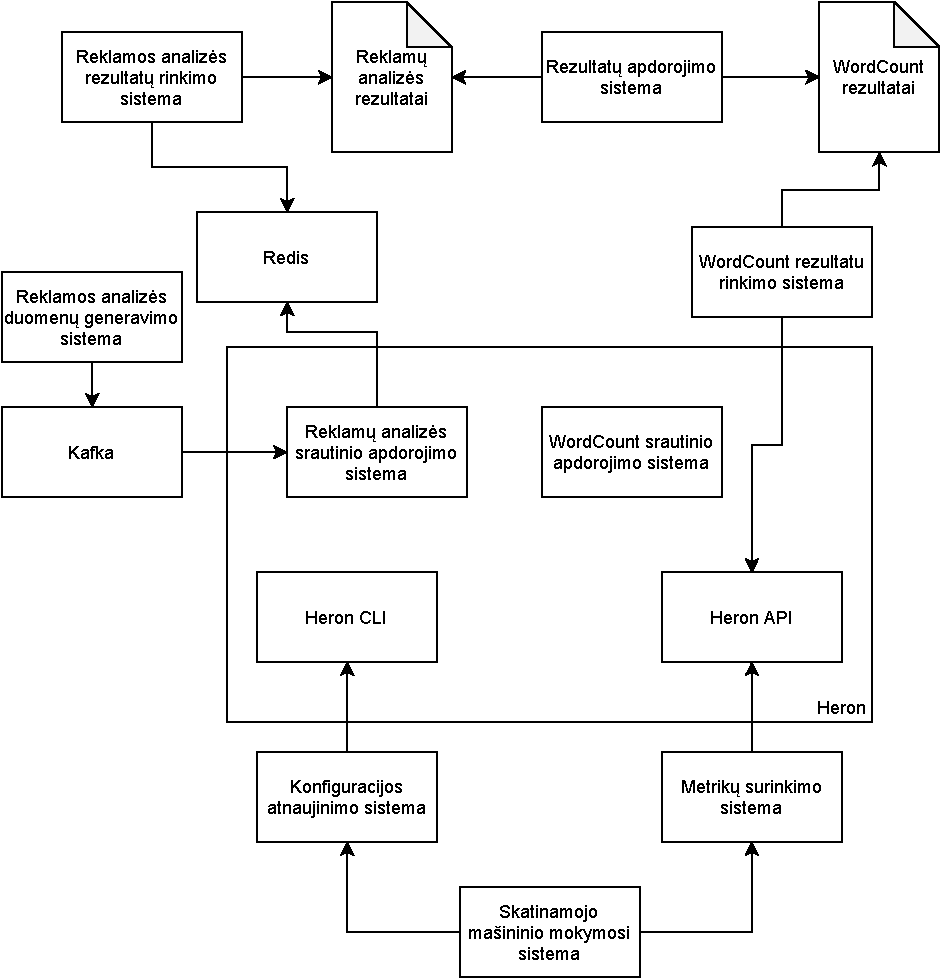
\includegraphics[width=14cm]{img/Experiment.pdf}
    \caption{Eksperimento atlikimo sistema}
    \label{experiment}
\end{figure} 

Sistemos, kurios reikalingos ekeperimetui:
\begin{enumerate}
    \item Skatinamojo mašininio mokymosi sistema. Kadangi bus atlikti bandymai su dviem skatinamojo mokymosi algoritmais: Deep Q Network ir Soft Actor Critc, bus parašyti du mašininio mokymosi agentai naudojant Python su PyTorch biblioteka. Taip pat bus suskurta aplinka aprašanti srautinio apdorojimo sistemos konfiguraciją. 
    \item Metrikų surinkimo sistema parašyta su Python naudojanti HTTP, kad gauti duomenis iš Heron API.
    \item Konfiguracijos atnaujinimo sistema parašyta su Python, kuri per Heron CLI pateikia atnaujinta konfiguraciją.
    \item Reklamų srautinio apdorojimo sistema parašyta su JAVA, gaunanti duomenis iš Kafka žinučių eilės ir sauganti rezultatus Redis duomenų bazėje.
    \item WordCount srautinio apdorojimo sistema parašyta su JAVA, pati generuojanti duomenis ir nesauganti duomenis į išorę. 
    \item WordCount rezultatų sistema parašyta su Python skaitanti vėlinimo metrikas iš Heron API ir sauganti rezultatus tekstiniame faile.
    \item Rezultatų apdorojimo sistema parašyta su Python, kuri surenka duomenis iš rezultatų failų, apdoroja  juos ir gražina skirtingų sprendimų diagramas.
    \item Reklamos analizės rezultatų rinkimo sistema parašyta su Clojure ir pateikta kartu su Reklamos analizės greitaveikos testu.
    \item Reklamos analizės duomenų generavimo sistema parašyta su Clojure ir pateikta kartu su Reklamos analizės greitaveikos testu.
\end{enumerate}

Kompiuterinės įrangos su kuria bus atliekamas eksperimentas parametrai:
\begin{itemize}
    \item Procesorius: Intel Core i7-5930k (6 branduoliai/12 gijų)
    \item Operatyvi atmintis: 64 GB (2666 MHz)
    \item Vaizdo plokštė: Nvidia GTX 1080Ti
    \item Operacinė sistema: Windows 10 Education
\end{itemize}

Kadangi Heron nepalaiko Windows sistemos visi tyrimai ir visos reikiamos posistemės leidžiamos naudojant Windows Subsystem Linux (toliau WSL) su Ubuntu 18.04. WSL yra suderinamumo sluoksnis naudojantis Linux branduolį per Hyper-V, kieno pagalba galima leisti programas skirtas Linux be emuliacijos ir taip neprarasti greitaveikos.

Pagrindinės programinės įrangos versijos:
\begin{itemize}
    \item Apache Heron: 0.20.3
    \item Kafka: 2.13
    \item Redis: 4.0.9
    \item Python: 3.6.9
    \item Java: 8
\end{itemize}
\subsection{Planuojamų eksperimentų apimtis}

Magistro darba eksperimentai bus atliekami su keturiais skirtigais sprendimais:
\begin{itemize}
    \item Srautinio apdorojimo sistemos veikimas su standartine konfiguracija.
    \item Srautinio apdorojimos sistemos veikimas balansuojant ją naudojant sukurtą eksperimentinį sprendimą pagal apibrėžtą balansavimo algoritma naudojant:
    \begin{itemize}
        \item REINFORCE algortimą skatinamojo mokymosi posistemėje.
        \item Deep Q Network algoritmą skatinamojo mokymosi posistemėje.
        \item Soft Actor Critic algortimą skatinamojo mokymosi posistemėje.
    \end{itemize}
\end{itemize}

Kiekvienas sprendimas bus testuojamas su dviem srautinio apdorojimo sistemų implementacijomis:
\begin{itemize}
    \item Reklamų analizės srautinio apdorojimo sistema.
    \item WordCount srautinio apdorojimo sistema.
\end{itemize}

Reklamų analizės sistema rezultatus talpina tekstini failą, kur kiekvienas įrašas yra vėlinimas milisekundėmis nuo paskutinio išsiųsto įrašo į žinučių eilę tam specifiniam kampanijos langui iki kol jis yra įrašomas į Redis duombazę. WordCount sistemos rezultatai bus skaitomi tiesiai iš Heron platformos naudojant Heron API ir saugomi į failą tokiu pačiu formatu kaip ir reklamų analizės sistema, naudojant absoliutų vėlinimą gauta iš Heron API. 

Eksperimentai su visomis sistemomis bus vykdomi po 10 valandų, kadangi \cite{vaquero2018autotuning} straipsnio autoriai nustatė, kad jų balanasavimo algoritmas konverguoja po maždaug 11 valandų. 
Gauti rezultatai iš failo bus skaitomi pasirašyta Python programa, kuri apdoroja duomenis į dvi grupes: visų sprendimų vėlinimą ir visų sprendimų vėlinimo 99–tą percentilę ir sugeneruoja linijinas diagramas, kiekvienai vėlinimo grupei pagal sprendimą.

Taigi iš viso magistro darbe planuojama atlikti 8 eksperimentus, kurių bendra trukmė – 80 valandų.


\sectionnonum{Rezultatai ir išvados}

\subsection*{Rezultatai}
\begin{enumerate}
    \item Apibrėžtas srautinio apdorojimo sistemos valdymo modelis, naudojanat skatinamajį mašininį mokymasį. 
    \item Apibrėžtas balansavimo algoritmas, jo įeitis ir rezultatai.
    \item Aprašyta eksperimento eiga ir reikalavimai eksperimentinei sistemai.
\end{enumerate}
\subsection*{Išvados}
\begin{enumerate}
    \item Apibrėžtas modelis yra įgyvendinamas ir modelio naudojamo algoritmo validumą įmanoma patikrinti atlikus eksperimentus ir palyginus rezultatus.
    \item Apibrėžus eksperimentine sistema matome, jog eksperimentas yra validus, įgyvendinamas ir atlikus eksperimentą rezultatus galima surinkti bei įvertinti.
\end{enumerate}
\printbibliography[heading=bibintoc] 

\end{document}
